%%
\section{Stateful Tracking}
\label{sec:stateful-tracking}
%%
The most straightforward approach to tracking a user involves storing a unique identifier in their browser and retrieving it or modifying it as they browse different websites, which is a process known as ``stateful tracking''. 
%
Browsers provide a number of interfaces (\eg{}, cookies) that are designed to associate \textit{state} to the user's visit. 
%
Browsers also provide many interfaces that store information as a side effect of some other functionality provided to the website (\eg{}, E-Tags, HSTS upgrades), which trackers can sometimes abuse to encode a unique identifier~\cite{englehardtAutomatedDiscoveryPrivacy2018,ashkansoltaniFlashCookiesPrivacy2011,solomosTalesFaviconsCaches2021}.
%
In this section, we first describe third-party stateful tracking (\autoref{sec:tp-stateful}) and next its evolution towards first-party stateful tracking (\autoref{sec:fp-stateful}).
%
We conclude by discussing the defenses that exist against these stateful tracking mechanisms in~\autoref{sec:stateful-defenses}.

%%
\subsection{Third-party Stateful Tracking}
\label{sec:tp-stateful}

Krishnamurthy and Wills provided much of the early insight into the prevalence and growth of third-party stateful tracking. 
%
In 2006, they found third-party resources present on more than half of the sites, however the network of trackers was still relatively fragmented back then, with only three cookie-bearing third-party domains present on more than 10\% of sites~\cite{krishnamurthyGeneratingPrivacyFootprint2006}. 
%
In 2009, they documented the rapid growth of trackers, and showed how acquisitions allowed the largest trackers to have visibility on 10-60\% of sites~\cite{krishnamurthyPrivacyDiffusionWeb2009}. 
%
In the following years, researchers have shown a continual growth in the presence and diversity of third-party stateful tracking~\cite{soltaniFlashCookiesPrivacy2009,roesnerDetectingDefendingThirdparty2012,mayerThirdPartyWebTracking2012,acarFPDetectiveDustingWeb2013,eubankShiningFloodlightsMobile2013, altaweelWebPrivacyCensus2015,englehardtOnlineTracking1millionsite2016,lernerInternetJonesRaiders2016,schelterUbiquityWebTracking2018} and documented the rise and fall of different players in the ecosystem and behaviors (\eg{}, popup-based trackers declining after browsers blocked popups by default)~\cite{lernerInternetJonesRaiders2016}.
%
As of 2025, stateful tracking is ubiquitous: third parties are present on nearly every site and large-scale tracking networks are common---with top 35 trackers present on 10\% or more of the web~\cite{duckduckgoTrackerRadarWiki2024}.


\subsubsection{Cookies} Cookies---first specified by Lou Montulli at Netscape in the mid-1990s---constitute one of the most popular stateful tracking mechanisms. 
%
The origin of cookies initially stemmed from the need to maintain a state when the browser communicates with a web server via HTTP, a stateless protocol~\cite{kristolHTTPCookiesStandards2001}. 
%
Cookies essentially store a small bit of text in the user’s browser associated with a specific web domain. 
%
For example, a website can store a user’s authentication token in their browser via a cookie, which is then presented to the web server with each request that the user’s browser makes, allowing the website to verify the user’s authentication status. 
%
Based on the cookies' attributes and the diverse access control policies implemented by web vendors, browsers mediate which resources and domains are able to access specific cookies~\cite{beugin2024WebAlmanac2024,singhIncoherenciesWebBrowser2010,mdnSameoriginPolicySecurity2024}.

\begin{figure}
    \centering
    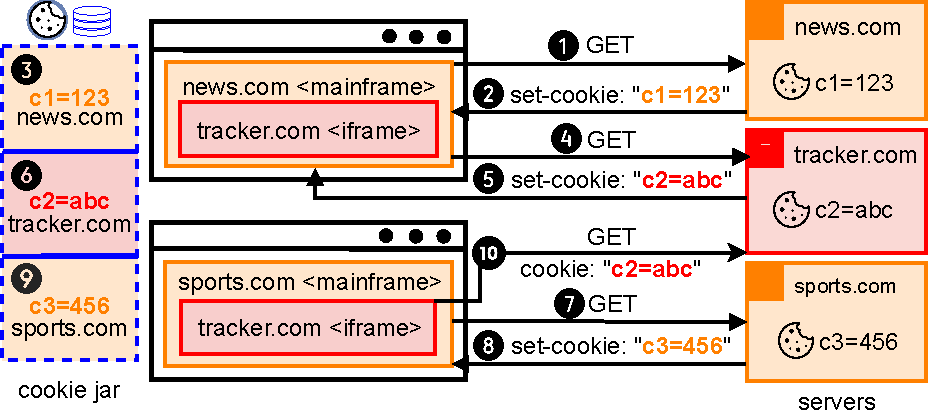
\includegraphics[width=1\linewidth]{figures/tracking-mechanisms-cookie.pdf}
    \caption{Cookie-based Tracking}
    \label{subfig:cookie-tracking}
\end{figure}

%%
First- or third-party domains on a webpage can set and receive cookies---either via \texttt{cookie} and \texttt{set-cookie} headers in network requests and responses respectively or via the \texttt{document.cookie} JavaScript method. 
%
In a first-party context, cookies allow a user to be re-identified to the website that they visit, while in a third-party context, it allows for cross-site tracking. 
%
For example, in \autoref{subfig:cookie-tracking}, \texttt{news.com} and \texttt{sports.com} both include iframes with ads from \texttt{tracker.com}. 
%
As a result, the user’s browser will send the same \texttt{tracker.com} cookie with requests to load the iframes on both pages. 
%
On \texttt{tracker.com} server's side, these two requests can be attributed to the same user and combined with additional information about the user-visited website. 
% (from the HTTP Referrer header or query parameters passed along when the request to load the iframe is made). 
%
Privacy concerns with third-party cookies were identified as early as their introduction~\cite{montulliHTTPStateManagement1997,kristolHTTPCookiesStandards2001} as public concern over web tracking elevated to the point where the FTC held a workshop on the topic in 1997~\cite{ftcWorkshopConsumerInformation1997} and the United States government audited and banned the use of cookies on government websites~\cite{SenatorRaisesPrivacy2001}. 
%
Nonetheless, this mechanism has been the dominant form of web tracking for many years.







%%
%%
\subsubsection{Cookie Syncing}
%%
Third-parties included on a few websites, are only able to track users across that limited number of sites~\cite{roesnerDetectingDefendingThirdparty2012,lernerInternetJonesRaiders2016}. 
%
Moreover, under the SOP restriction, a third-party on a webpage cannot share its cookies with another third-party domain by directly initiating a request to it.
%
To overcome these constraints and exchange information collected about the user on different websites, third-party companies rely on cookie syncing or cookie matching~\cite{acarWebNeverForgets2014,englehardtOnlineTracking1millionsite2016,bashirTracingInformationFlows2016,papadopoulosCookieSynchronizationEverything2019,fouadMissedFilterLists2020,urbanMeasuringImpactGDPR2020}---first described by Olejnik et al.~\cite{olejnikSellingPrivacyAuction2014} and also named as ``referred tracking'' by Roesner et al.~\cite{roesnerDetectingDefendingThirdparty2012}. 

\begin{figure}[htbp]
    \vspace{-3mm}
    \centering
    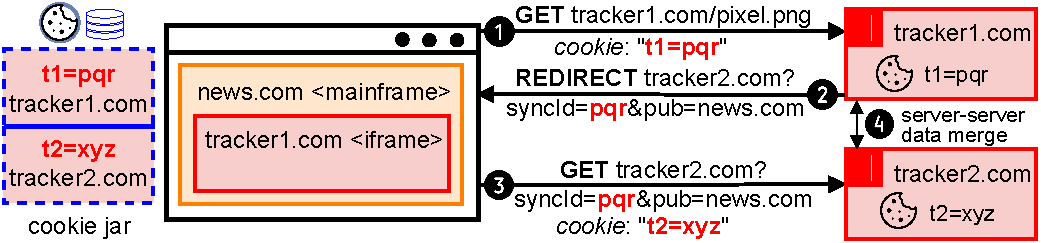
\includegraphics[width=1\linewidth]{figures/tracking-mechanisms-cookie-syncing.pdf}
    \caption{Cookie Syncing}
    \label{subfig:cookie-syncing}
    \vspace{-2mm}
\end{figure}

%%
This mechanism relies on synchronizing user identifiers known to two different third parties that are typically stored in third-party cookies and most commonly communicated via URL parameters. 
%
Following from the previous example, let’s suppose there are two trackers---\texttt{tracker1.com} and \texttt{tracker2.com}. 
%
If only \texttt{tracker1.com} is present on \texttt{news.com} as shown in \autoref{subfig:cookie-syncing}, it can share its user identifier stored in a third-party cookie by initiating a request to \texttt{tracker2.com} and adding it in the URL parameter. 
%
This would allow \texttt{tracker2.com} to know the identifier the user has for \texttt{tracker1.com}, match it with the user identifier of \texttt{tracker2.com}, and communicate server-to-server to further merge the information collected about this user by \texttt{tracker1.com} and \texttt{tracker2.com}. 




%%
\begin{table*}[ht]\small
\centering
\caption{Common use cases of third-party tracking pixels (tags) on websites.}
\label{tab:tracking-tags-usecases}
\renewcommand{\arraystretch}{1.3} % Adds vertical padding for improved readability
\begin{tabular}{@{}p{2.65cm} p{9.7cm} p{4.6cm}@{}}
\toprule
\textbf{Use Case} & \textbf{Purpose} & \textbf{Example Pixel Providers} \\
\midrule
Analytics & Measures site traffic to inform site improvements and business decisions & Google Analytics (GA); Mixpanel \\[4pt]
\hline
Remarketing & Builds audiences of past visitors for (re)targeted advertising & Meta Pixel; TikTok Pixel \\[4pt]
\hline
Conversion Tracking & Attributes conversions to ad campaigns to measure/optimize ad performance & Google Ads Conversion Tag \\[4pt]
\hline
Tag Management & Allows deployment of multiple tags via one container & Google Tag Manager; Tealium iQ \\[4pt]
\hline
Bot Detection & Detects and filters bot activity by analyzing user behavior and environment & Cloudflare; reCAPTCHA \\[4pt]
\hline
Session Replay & Records and replays individual user sessions for UX analysis & Clarity; Hotjar \\
\bottomrule
\end{tabular}
\end{table*}



%%
\subsubsection{Tracking Tags}
%%
Traditionally, tracking pixels (also called invisible pixels) used to be basic 1x1 image elements embedded on a webpage that pointed to some tracking endpoint.
%
When a user visits a webpage embedding a 1x1 pixel, user data is shared with the tracker, allowing user tracking on the same site as well as cross-site.
%
Image-based tracking pixels have been primarily used for analytics, ad (re)targeting, and conversion tracking. 
%
Researchers have conducted various large-scale measurements to study image-based tracking pixels \cite{Narayanan2017WebtapSpringer,englehardtOnlineTracking1millionsite2016,lernerInternetJonesRaiders2016, bekosHitchhikersGuideFacebook2023, agarwal2021under,vekaria2021differential}.

\begin{figure}[htbp]
    \vspace{-2mm}
    \centering
    
\includegraphics[width=1\linewidth]{figures/tracking-mechanisms-tracking-tags.pdf}
    \caption{Tracking Scripts}
    \label{subfig:tracking-scripts}
    \vspace{-2mm}
\end{figure}

%%
Over the years, tracking pixels have significantly advanced in their capabilities.
%
Modern tracking pixels, also referred to as tracking tags, rely on JavaScript to collect more fine-grained information in browsers. 
%
\autoref{subfig:tracking-scripts} represents a simple scenario where a tracking pixel from \texttt{tracker.com} is embedded on the homepage as well as on the \texttt{/signup} page of \texttt{news.com}, respectively collecting and sharing button clicks and form events with its own server, with the help of its tracking script.
%
Thus, as summarized in \autoref{tab:tracking-tags-usecases}, tracking pixels have expanded in scope to support additional use cases, such as managing multiple pixels via a single tag, bot detection, and replaying of user sessions.





%%
\subsection{First-party Stateful Tracking}
\label{sec:fp-stateful}

%%
When browsers block or partition third-party access (by origin) to stateful APIs, trackers aren’t able to store and retrieve identifiers \textit{across} sites. 
%
At best, when storage is partitioned they will be able to track a user’s activity on a single site, as any identifiers they write to partitioned storage will not be accessible on any other websites. 
%
% We further discuss this in~\autoref{sec:stateless-defenses}.

%%
To circumvent these protections, trackers embed third-party scripts in the first-party context to set and sync first-party identifiers that aid in tracking of a users’ same-site activity with cross-site activity. 
%
Trackers have also turned to passing information across sites during page navigations through so called ``Navigational Tracking''~\cite{snyderNavigationalTrackingMitigations2024}. 
%
Tracking information passed during navigations can be persisted on each site using first-party storage or partitioned third-party storage, depending on how the tracker is embedded. 
%
% Likewise, trackers can also abuse Stateless Tracking techniques (\autoref{sec:stateless-tracking}) to identify users across sites and persist that information in storage scoped to the first party site. We discuss these approaches in more detail in this section. \\

%%
\subsubsection{Cookies}
\label{subsubsec:stateful-tracking-cookies}
%%
When third-party tracking scripts are embedded into first-party execution contexts, the scripts execute with the same privileges as first-party scripts. 
%
This allows those scripts to read and write JavaScript-accessible first-party storage as if they were a first-party script~\cite{bahramiCOOKIEGUARDCharacterizingIsolating2024}. 
%
Nearly 90\% of sites have first-party tracking cookies set by third-party scripts~\cite{munirCookieGraphUnderstandingDetecting2023}. 
%
First-party cookies often store unique user identifiers created with browser fingerprinting as well as identifiers which are bounced through navigational tracking (see details below). 
%
Recent research has shown that trackers are increasingly using the first-party cookie jar~\cite{munirCookieGraphUnderstandingDetecting2023,vekaria2024WebAlmanac2024}. 
%
For example Google and Facebook set first-party analytics and tracking cookies on nearly half (49.48\%), and more than a quarter (28.76\%) of the most popular 12.7 million websites visited in Google Chrome~\cite{vekaria2024WebAlmanac2024}. 
%
Nearly 90\% of all websites use at least one tracking first party cookie and 96\% of these tracking cookies are in fact set by third-party scripts which are running in a first-party context.

%%
\subsubsection{Cookie Syncing}
%%
One of the privacy issues with first-party cookies is syncing of these stored identifiers with other third-parties. 
%
This sharing---first described by Fouad et al.~\cite{fouadMissedFilterLists2020}---allows third-parties to collude with each other and benefit from information gathered from users’ across different websites. 
%
In some cases, Google and Facebook set first-party cookies are shared with hundreds of other third-party domains~\cite{munirCookieGraphUnderstandingDetecting2023}. 
%
Using first-party cookies not only diminishes the privacy benefits achieved by blocking third-party cookies, but also introduces serious security issues, as first party cookie jars often contain sensitive user information, such as session identifiers used by SSO services~\cite{bahramiCOOKIEGUARDCharacterizingIsolating2024}. 
%
In addition to syncing first-party cookies, trackers also combine personal information obtained from users across different websites to create extensive identity graphs of users as described in~\autoref{sec:id-providers} to track users in absence of third-party cookies.

%%
\subsubsection{Tracking Tags}
%%
Image-based tracking pixels primarily rely on third-party cookies shared as part of fetch request of the image to track a user.
%
Blocking third-party cookies render tracking pixels embedded as image elements ineffective. 
%
However, modern tracking tags relying on JavaScript can still be used to track users in a first-party context~\cite{munirCookieGraphUnderstandingDetecting2023}. 
%
These tags are often included in the main frame context of a website by the developer, allowing pixel tracking companies to monitor different user activities using first-party execution privileges.


%%
\subsubsection{Navigational Tracking}
%%
A popular mechanism for sharing identifiers is via link decorations as depicted in \autoref{subfig:navigational-tracking}. 
%
Recent research has identified query parameters, resource paths, and URL fragments being used for sharing user data, such as first-party cookies and email addresses, on more than 70\% of websites~\cite{munirPURLSafeEffective2024}, in absence of third-party cookies or first-party partitioning. 
%
Besides link decorations, bounce tracking is another navigation-based mechanism that allows trackers to read/write their cookies across sites, rendering third-party cookie blocking ineffective~\cite{kellyBounceTrackingMitigations2022}. 


\begin{figure}[htbp]
    \vspace{-2mm}
    \centering
    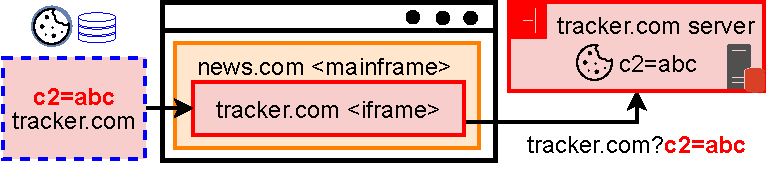
\includegraphics[width=1\linewidth]{figures/tracking-mechanisms-navigational-tracking.pdf}
    \caption{Navigational Tracking}
    \label{subfig:navigational-tracking}
    \vspace{-2mm}
\end{figure}

%%
At a high level, a tracker’s goal is to momentarily surface or visit its own domain in the browser’s \emph{first-party} context, because this lets it read and write identifiers that persist in first-party storage. 
%
\autoref{subfig:bounce-tracking} shows a typical \textbf{bounce-tracking} sequence:
%
\ding{182} A third-party script on \texttt{news.com} reads first-party identifier(s) stored under \texttt{news.com} and
%
\ding{183} includes them in the request to \texttt{tracker.com}.
%
\ding{184} Browser redirects to \texttt{tracker.com}—either by a user click or automatically (e.g., \texttt{window.location.href="...";} or a \texttt{<meta http-equiv="refresh">}).
%
\ding{185} Once loaded as a \emph{first party}, \texttt{tracker.com} reads the identifier from the URL or merges it with an existing cookie, rewriting the URL to its final destination (e.g., back to \texttt{news.com} or a different domain), embedding the consolidated identifier.
%
\ding{186} The browser navigates to \texttt{news.com}; the tracker’s script there extracts identifier from the decorated URL and 
%
\ding{187} stores it in \texttt{news.com}’s first-party storage, completing the cross-context linkage (if redirected to same first-party) or cross-site linkage (if redirected to a different domain).


\begin{figure}[htbp]
    \vspace{-2mm}
    \centering
    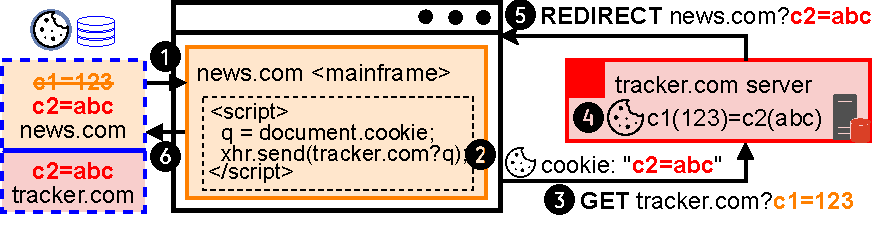
\includegraphics[width=1\linewidth]{figures/tracking-mechanisms-bounce-tracking.pdf}
    \caption{Bounce Tracking}
    \label{subfig:bounce-tracking}
    \vspace{-2mm}
\end{figure}

Bounce chains can involve two sites—\texttt{news.com} → \texttt{tracker.com} → \texttt{news.com}, or longer—allowing the tracker to propagate a stable user identifier across multiple seemingly unrelated websites despite third-party cookie restrictions.
%
% As a result of this process, a tracker is able to use the same identifier across websites. 
%
Due to potential usability disruptions and the implementation of defensive measures, bounce tracking is not widely pervasive
\cite{iqbalKhaleesiBreakerAdvertising2022}.
%
Measurements in 2020 found that 11.6\% of sites use one of the top 100 redirectors~\cite{koopInDepthEvaluationRedirect2020}, and in 2022 such identifiers were present in 8.1\% of the crawled navigations~\cite{randallMeasuringUIDSmuggling2022}.
%and in 2024 that nearly three-quarters of 20k sampled top websites abuse link decoration~\cite{munirPURLSafeEffective2024}.


%%
\subsection{Defenses Against Stateful Tracking}
\label{sec:stateful-defenses}

Given the broad adoption of stateful tracking and its perceived intrusive nature, numerous tracking countermeasures have been proposed by the research community, some of which have either been adopted by browsers or are available to users through browser extensions.

%%
\vspace{-4mm}
\subsubsection{Third-party Stateful Tracking Protections}

%%
\paragraph{Clearing Cookies.}
Logically, a user could clear the cookies in their browser at the end of each session to protect themselves from being tracked. 
%
However, browser cookie clearing features do not typically clear \textit{all} stateful mechanisms provided to sites \cite{acarWebNeverForgets2014, englehardtOnlineTracking1millionsite2016}. 
%
For example, clearing cookies often does not remove identifiers stored in browser storage APIs \texttt{localStorage}~\cite{ayensonFlashCookiesPrivacy2011,roesnerDetectingDefendingThirdparty2012}, \texttt{IndexedDB}~\cite{acarFPDetectiveDustingWeb2013}, E-Tags~\cite{ayensonFlashCookiesPrivacy2011} and browser cache~\cite{sorensenZombiecookiesCaseStudies2013}
%
A malicious tracker can take advantage of this limitation by storing copies of their tracking identifiers in locations that aren’t cleared by the browser. 
%
Once a user clears their cookies, the tracker can use that hidden information to ``respawn'' or reconstruct the user’s identifier, creating a so-called ``supercookie'' or ``evercookie''~\cite{ayensonFlashCookiesPrivacy2011,soltaniFlashCookiesPrivacy2009,fouadMyCookiePhoenix2022}.
%
The most publicized example of supercookie was the Adobe's Flash browser plugin that provided no mechanism for browsers to clear its storage \cite{soltaniFlashCookiesPrivacy2009,solomosTalesFaviconsCaches2021}.
%
Any API that allows a tracker to persist state to the user’s device is a potential supercookie vector~\cite{aliNavigatingMurkyWaters2023}. 
%
Even just a single bit of storage can be abused if a tracker is able to string together multiple calls to an API, each encoding another bit from the identifier. 
%
Samy Kamkar first demonstrated how widespread this risk by encoding identifiers in APIs like HTTP Strict Transport Security (HSTS), Web Cache, \texttt{window.name}, and Web History~\cite{kamkarSamyKamkarEvercookie2010}. 
%
Variants of the same attack were also demonstrated later on other browser APIs~\cite{klink1334485TrackingUsing2017,goodinUnpatchedBrowserWeaknesses2015,evansPublicKeyPinning2015}. 
%
Ultimately supercookie risk was the prime motivation behind the network and storage partitioning efforts of Firefox, Chrome, and Safari~\cite{menkeStorageIsolationProject2020,privacycommunitygroupClientSideStoragePartitioning2022,mdnStatePartitioningPrivacy2024}. 
%
As of 2025, most browsers have blocked or partitioned third-party access to stateful APIs, preventing those APIs from being used to track users across websites.

%%
\vspace{-1mm}
\paragraph{Restrictions on Third-party Cookies.}
%
Browser vendors attempt to block most third-party cookies~\cite{mdnThirdpartyCookiesPrivacy2024} but leave some exceptions to support non-tracking use cases such as cookies that enable single sign-on (SSO), whose removal may lead to website breakage \cite{crouchImprovingPrivacyBreaking2018}. 
%
Privacy-focused browsers, such as Brave~\cite{braveBrowserThatPuts}, apply the most aggressive restrictions by blocking all third-party cookies by-default and allowing third-parties to share a partitioned ephemeral storage for the lifetime of the browsing session \cite{braveprivacyteamEphemeralThirdpartySite2021}. 
% (\ie{}, until the browser is closed or the last instance of first-party website (eTLD+1) closes)~\cite{braveprivacyteamEphemeralThirdpartySite2021}.
%
Among the mainstream browsers, Safari~\cite{appleSafari} and Firefox~\cite{mozillaGetFirefoxBrowser} have the most effective restrictions. 
%
Safari currently blocks all third-party cookies unless the domain (eTLD+1) has been visited by the user as a first-party or if the third-party explicitly requests to use the cookies through the Storage Access API~\cite{TrackingPreventionWebKit2020}. 
%
It further relies on an ML model to detect whether the domains with third-party access engage in tracking and restrict their cookies if the user has not interacted with the domain as a first-party in the last 30 days. 
%
Firefox blocks third-party cookies from known trackers (as determined by the Disconnect's tracking protection list~\cite{disconnectDisconnect}) and also partitions third-party cookies, such that each first-party and third-party origin combination has a separate cookie jar~\cite{mdnThirdpartyCookiesPrivacy2024}.
%
Initially, following in the footsteps of Safari and Firefox, Google Chrome~\cite{googleGoogleChromeFast} announced plans to block all third-party cookies~\cite{chromeBuildingMorePrivate2020}, which after several delays, it decided not to proceed with~\cite{chavezNewPathPrivacy2024}. 
%
Chrome currently offers various tools for developers to manage third-party cookies, including JavaScript APIs like the Storage Access API~\cite{mdnStorageAccessAPI2024} and cookie directives like the ``SameSite' attribute~\cite{mdnSetCookieHTTPMDN2024}. 
%
However, trackers may not adhere to or use these mechanisms. 
%
Moreover, they have migrated to alternative tracking techniques by circumventing existing protections.


\vspace{-1mm}
\paragraph{Blocking Trackers.}
%%
Filter lists are widely used by browsers (\eg{}, Brave) and browser extensions (\eg{}, uBlock Origin) to block third-party tracking requests.
%
However, filter list based ad or tracker blocking faces significant limitations: 
%
(1) manually curated lists are maintained by small community individuals and do not capture nuanced techniques. 
%
(2) as lists grow in size, they contain outdated or too narrow entries (\eg{} 90\% of EasyList rules are practically never triggered \cite{snyderWhoFiltersFilters2020}).
%
(3) being static, trackers keep evading them.
%
To overcome these challenges, researchers have focused on building ML-driven advertising or tracking request blockers ~\cite{iqbalAdGraphGraphBasedApproach2020, sibyWebGraphCapturingAdvertising2022, yangWTAGRAPHWebTracking2022, leAutoFRAutomatedFilter2023}.
%
AutoFR \cite{leAutoFRAutomatedFilter2023} proposes a fully automated framework for filter rule creation and evaluation.
%
While AdGraph \cite{iqbalAdGraphGraphBasedApproach2020}, WebGraph \cite{sibyWebGraphCapturingAdvertising2022}, and WTAGraph \cite{yangWTAGRAPHWebTracking2022} treat a webpage as a graph of HTML structure, network requests, and JavaScript behavior of a webpage to train a classifier for identifying and subsequently blocking advertising and tracking resources.
%
These approaches can generalize well to discover previously unknown trackers and adapt to evolving tracking behaviours. 
%
Brave implements an AdGraph-based ML solution (PageGraph) to detect and block trackers.
%
Beyond network requests, another popular anti-tracking method is to detect and block tracking scripts or JavaScript code at different granularities such as domain or path-based script blocking or function blocking within an otherwise benign script \cite{ikramSeamlessTrackingFreeWeb2016,alrizahErrorsMisunderstandingsAttacks2019,snyderWhoFiltersFilters2020,smithSugarCoatProgrammaticallyGenerating2021,chenDetectingFilterList2021,daoCNAMECloakingBasedTracking2021,leCVInspectorAutomatingDetection2021,amjadTrackerSiftUntanglingMixed2021,amjadBlockingJavaScriptBreaking2023,amjadBlockingTrackingJavaScript2024,ublockoriginUBlockOUBOScriptlets2025}.%
Adversarial trackers are incentivized to evade such blocking (\eg{} by changing script location or causing site breakage), posing challenges.


%%
\vspace{-4mm}
\subsubsection{Protections Against First-party Circumventions}

\paragraph{Restrictions on First-party Cookies.}
Unlike third-party cookies, first-party cookies cannot be as easily blocked completely because it would break critical website functionality such as maintaining login state. 
%
Therefore, they require more targeted countermeasures as listed below. 



%%
\vspace{-1mm}
\paragraph{Limiting the Lifetime of First-party Storage Written by Tracking Scripts.}
%
Safari’s Intelligent Tracking Protection (ITP) expires all first-party cookies or storage set by scripts post no user interaction for 7 days \cite{TrackingPreventionWebKit2020}. 
%
To mitigate workarounds that automatically overwrite cookies written by scripts with HTTP cookies, Safari detects third-party hosts cloaked under first-party subdomains using heuristics applied to the first-party host’s CNAME and IP address~\cite{TrackingPreventionWebKit2020}. 
%
Brave implements a limited version of this which caps the lifetime of cookies set by scripts to 7 days~\cite{bravePrivacyProtectionSecurity}. \\



%%
\vspace{-4mm}
\paragraph{Removing or Limiting the Persistence of Identifiers Passed in URL Parameters.}
%
Several browsers remove URL parameters known to be used by trackers. 
%
Firefox~\cite{mozillaQueryParameterStripping} implements removal in a non-default mode, while Brave~\cite{braveprivacyteamGrabBagQuery2020} and DuckDuckGo~\cite{duckduckgoDuckDuckGoWebTracking} ship it by default. 
%
When URL parameters are removed on navigation, tracking scripts embedded in the first-party context are prevented from accessing tracking IDs across sites. 
%
Safari takes a different approach: instead of removing tracking parameters, it limits the lifetime of script-accessible storage from 7 days to 24 hours when ITP detects link decoration~\cite{TrackingPreventionWebKit2020}.



%%
\vspace{-1mm}
\paragraph{Limiting First-party Storage Set During a Bounce.}
%
Bounce tracking not only circumvents third-party storage protections but also allows unrestricted access to tracker’s first-party storage. 
%
Browsers mitigate it by differentiating between a \textit{legitimate visit} to a site and a brief \textit{bounce} for tracking purposes. 
%
The fact that some authentication flows appear similar to bounce tracking complicates it~\cite{kellyBounceTrackingMitigations2022}. 
%
Brave and Firefox use blocklists to detect potential bounce trackers, whereas Safari and Chrome use heuristics based on site behavior as mitigations~\cite{snyderNavigationalTrackingMitigations2024}. 
%
Firefox, Chrome, and Safari delete all site storage for these domains unless there's an evidence of legitimate and recent user interaction with the site; the definition of \textit{legitimate} and \textit{recent} varies by browser~\cite{snyderNavigationalTrackingMitigations2024,TrackingPreventionWebKit2020}. 
%
While Brave provides suspected bounce trackers with access to ephemeral storage that’s cleared once all tabs opened from that tracker are closed, so long as the tracker doesn’t already have persistent storage set~\cite{braveprivacyteamUnlinkableBouncingMore2022}.

\vspace{-1mm}
\paragraph{Blocking First-party Cookies.}
Privacy-enhancing extensions support targeted deletion of known tracking cookies, including first-party cookies, through a filter list \cite{ublockResourcesLibrary,adguardrteamScriptletsWikiAboutscriptletsmd,schininaSourceBehavioralCookieremoverjs2024}.
%
While the filter lists face aforementioned challenges, they can also be automatically curated using a ML-based approach \cite{munirCookieGraphUnderstandingDetecting2023,bollingerAutomatingCookieConsent2022,schoniBlockCookiesNot2024a}.